
% this file is called up by thesis.tex
% content in this file will be fed into the main document
    \graphicspath{{Background_Folder/figures/PNG/}{Background_Folder/figures/PDF/}{Background_Folder/figures/}}

%: ———————-- introduction file header ———————--
\chapter{Background}
        This chapter provides the necessary background technical knowledge required to understand the main results of this thesis and their implications to related fields of physics. These include both the theoretical framework we will use and the real world phenomena to which it relates to. As should already be clear by now, in this text, we will concern ourselves with the study of planar systems at finite density. We will approach the study of these two dimensional systems through the framework of Quantum Field Theory (QFT). 

    There are two important aspects of QFT that will play a major role for us. One of them is the relation between the grand canonical statistical partition function and QFT. The other aspect is the distinct way in which the gauge principle manifests itself in 2+1 dimensional theories. The latter is addressed in \ref{CS_sec}, where we review the basics of \textit{Chern-Simons theory}. The former is discussed in \ref{GCE_sec}, where we will spend time reminding ourselves some basic statistical mechanics. 

   % After we have covered these, we will turn to the physics this formalism aims to address in \ref{phys_app_sec}. We will review the \textit{Landau-Ginzburg  paradigm} \ref{Landau-Ginzburg_sec} of symmetry breaking and phase transitions, its inability to account for all phases observable in nature and where topological phases of matter fit in this picture.

    After we have covered these, , we will spend some time looking at the problems of the \textit{fractional and integer quantum hall effects} (FQHE/IQHE) in \ref{FQHE_sec} and emphasize its relation to Chern-Simons matter theories. This will help us understand the applications and motivate the study of the models we are concerned with in this text.

    Then, we shall continue by reviewing the properties of \textit{vortices} in section \ref{vortices_sec}. Specifically, we look at vortices in the abelian Higgs model, Pure abelian Chern-Simons theory with scalar matter and the mixed case where both $S_{\text{Maxwell}}$ and $S_{\text{CS}}$ play a role. We emphasize the importance of a \textit{BPS} bound for these systems. Finally, we discuss some subtleties relating to non-abelian vortices.

    We continue by addressing \textit{Fermi-Bose and particle-vortex dualities} in \ref{Fermi-Bose_sec}, which were the primary motivation for this work. We provide the relevant information about CFTs and RG flows in order to keep the presentation self-contained. We outline important aspects of the dualities in order to highlight where our work fits in that context.

    Finally, we include a section concerning the physics of \textit{non-commutative} field theory, its relation to the theory of fluids, in particular, the description of the Quantum Hall fluid in terms of a \textit{'fuzzy'} underlying space, in which the coordinates do not commute. We shall see that this description is a Chern-Simons theory and it seems to arise naturally out of the ground state in the finite density non-abelian model that we have studied.

        \section{Chern-Simons Theory} \label{CS_sec}
    Chern-Simons (CS) theory is a very unusual type of QFT both in its origin and its applications. It is a testament to the power and universality of mathematics, first conceived of as an abstract tool in the theory of differential operators and their connections to topology, it has grown to encompass many facets of modern physics and mathematics. From the computation of knot invariants to the prediction of non-abelian anyons, which are the ingredients necessary for performing a topological quantum computation -- currently one of the most promising approaches to fault tolerant quantum computation, due to the topological stability of the qubits. It is an example of a topological field theory (TQFT), which means that it is independent of the metric and so any observable is related to a topological invariant. It is the basis for three dimensional gravity \cite{gr-qc/0503022}, provides a field theoretic explanation for the Quantum Hall Effect and anyonic physics \cite{cond-mat/9501022, 1606.06687}, has been instrumental in the classification of rational 2D CFTs \cite{Moore1989}, creates a bridge between theoretical physics and knot theory \cite{Witten1989} and, recently, it has uncovered an equivalence between two types of matter, previously thought to have been fundamentally different -- namely Fermi-Bose duality \cite{1512.00161}. These are among the most noteworthy applications of CS theory. Therefore, in this section we justly take the time to review essential aspects of CS theory. Most of the results seen in this section, can also be found in the excellent review by Dunne \cite{hep-th/9902115}.

    In the study of fundamental physics, we should assume that any term in the Lagrangian that is not forbidden by a basic principle (\textit{e.g.} a symmetry or gauge-invariance) should be included in order to account for all aspects of the system at hand. From gauge theory we are familiar with the idea of introducing a gauge field to render a Lagrangian gauge invariant and then include a gauge-invariant Yang-Mills term that is responsible for the dynamics of the gauge potential. Modulo subtleties, this is true in any number of dimensions. Taking these subtleties into account, it turns out that in 2+1 dimensions, the Yang-Mills term is not the only gauge invariant term one can include. One can write down a term in the action, which is the integral of a three-form, depending solely on the gauge field $A_{\mu}$. This term, whilst not manifestly gauge invariant, leaves the partition function unchanged under gauge transfromations. This three-form is the Chern-Simons Lagrangian, which we write down here.

\begin{equation}
    {\mathcal{L}}_{CS}= \kappa \epsilon^{\mu\nu\rho} \  \mathrm{Tr} \left[ A_\mu\partial_\nu A_\rho +{2\over 3} A_\mu A_\nu A_\rho \right].
\label{cslag}
\end{equation}
The gauge field $A_\mu$ takes values in a finite dimensional representation of
the (semi-simple) gauge Lie algebra ${\mathfrak{G}}$. In an abelian theory, the gauge fields
$A_\mu$ commute, and so the trilinear term in \eqref{cslag} vanishes due to the
antisymmetry of the $\epsilon^{\mu\nu\rho}$ symbol. In the nonabelian case (just as in Yang-Mills theory) we write
\begin{align}
    A_\mu=A_\mu^a T^a,
\end{align}
 where the $T^a$ are the generators of ${\mathfrak{G}}$ (for $a=1,\dots dim({\mathfrak{G}})$), satisfying the commutation relations
 \begin{align}
    [T^a,T^b]=f^{abc}T^c,
 \end{align}
and the normalization 
\begin{align}
    \tr(T^a T^b)=-\frac{1}{2}\delta^{ab}.
\end{align}

We can define the field strength tensor in the usual way for a non-abelian gauge theory
\begin{align}
    F_{\mu \nu} = \partial_{\mu}A_{\nu} - \partial_{\nu} A_{\mu} + [A_{\mu}, A_{\nu}].
\end{align}




    $F_{\mu \nu}$ transforms in such a way that any expression that is the trace of a string of F's is gauge invariant. Since this Lagrangian is written in terms of $A_{\mu}$ as opposed to $F$, gauge invariance is no manifest.

    Before we delve into the details of the gauge invariance, it is helpful to venture into a quick digression about \textit{topology}. Topological invariants are such properties of spaces (and hence of field configurations defined on those spaces) that do not change under continuous transformations. And since most phenomena in the real world are continuous, we should expect that these invariants are important tools that we can use to better understand the physical world. Indeed, we shall see that these expectations are justified. 

    One way topologists use to classify spaces is through \textit{homotopy groups}. An example is the first homotopy group $\pi_1$ or the \textit{fundamental group}. This group is an indicator of the ``connectivity'' of a manifold. Its definition has to do with whether a given loop can be contracted to a point. More precisely, one can define a group at each point on a manifold, whose elements are equivalency classes of loops that start and end at that point \textit{and} are continuously deformable into each other. For example, if all loops on a given space can be contracted to a point, then the fundamental group $\pi_1$ is trivial, since all elements of the group are the identity. The group operation on these loops is such that we create a new loop from $g_1$ and $g_2$ by going around $g_1$ first, then followed by going around $g_2$. It turns out that loops that encircle a singular point (or hole in the space) $n$ times are \textbf{not} continuously deformable into loops that encircle said point $n'$ times, if $n \neq n'$. This is an intuitive way of understanding the fact that for each hole in the space-time manifold, the fundamental group acquires a cartesian factor of $\mathbb{Z}$. Meaning that loops can wind around singular points arbitrarily many integer number of times and the number of loops around one singular point is independent of the number around another.

    Such a classification is not restricted to loops but can also be applied to higher dimensional spheres. For example, the classes of mappings from the 3-sphere to 3-dimensional Euclidean space-time are classified by $\pi_3$. If $\pi_3$ is non-trivial, this tells us that not all gauge transformations are connected to the identity. Importantly for the purposes of theoretical physics, it is known that $\pi_3\left(SU(N) \right)$, $N\geq2$ is non-trivial. We shall now see how this fact plays a role in the gauge invariance of Chern-Simons.

    To convince ourselves of the gauge invariance, let us perform a gauge transformation
    \begin{align}
        A_{\mu} \rightarrow A'_{\mu} \equiv g^{-1} A_{\mu} g + g^{-1}\partial_{\mu} g
    \end{align}
    Under this transformation, the Lagrangian changes in the following way
    \begin{align}
        \mathcal{L}_{\text{CS}} &\rightarrow \mathcal{L}_{\text{CS}}  - \kappa \epsilon^{\mu \nu \rho} \partial_{\mu} \ \mathrm{Tr} \bigg[\partial_{\nu} g g^{-1} A_{\rho}  \bigg] - \frac{\kappa}{3} \epsilon^{\mu \nu \rho} \ \mathrm{Tr} \bigg[g^{-1} \partial_{\mu} g g^{-1} \partial_{\nu} g g^{-1} \partial_{\rho} g\bigg]
    \end{align}
    The first term is just a boundary term which vanishes. The second term turns out to be proportional to the \textit{winding density} of the gauge transformation, whose integral is an integer $N$ homotopy invariant.
    \begin{align}
        w(g) = \frac{1}{24 \pi^2} \epsilon^{\mu \nu \rho} \ \mathrm{Tr} \bigg[g^{-1}\partial_{\mu} g g^{-1} \partial_{\nu} g g^{-1} \partial_{\rho} g \bigg], \quad \int d^3x \ w(g(x)) = N \in \mathbb{Z}
    \end{align}
    Showing that the integral of this quantity is indeed a topological invariant is beyond the scope of this presentation. We refer the skeptical reader to the proof of Theorem 10.7 in Nakahara \cite{Nakahara}, which should at least provide some intuition.

    Gauge transformations with a non-zero winding number are called \textit{large gauge transformations}. Another way of saying this, is that they are mappings that are \textit{not} continuously connected to the identity transformation. Here we give an example to illustrate how these gauge transformations are different.
    Suppose we have a complex scalar field $\varphi$ defined on  $S^1$
    \begin{align}
        \varphi: S^1 \rightarrow \mathbb{C},
    \end{align}
    such that $\varphi = f(\theta) e^{i \alpha(\theta)}$, where $f\in \mathbb{R}$ and $\theta$ describes the position on the $S^1$. Here the $e ^{i \alpha (\theta)}$ can be absorbed into a $U(1)$ gauge transformation. Below (Fig \ref{large_gauge}) we have represented pictorially the phase of the scalar at a point on the manifold (in this case $S^1$) as a red arrow pointing in a direction on the plane. In (a) we have $\alpha(\theta) = \frac{\pi}{2}$. It is not hard to convince ourselves that we can transform this configuration to $\alpha(\theta) =0$ by making the same infinitesimal changes at every point on $S^1$. Thus $\alpha(\theta) = \frac{\pi}{2}$ is an example of the familiar kind of ``small gauge transformation''. One can go from (a) to (b) by setting $\alpha =\theta - \pi$. However, in this case we see that there is no way to make small transformations that are continuous. Configurations (b) and (c) are said to be in different homotopy classes, but they are in the same gauge equivalency class as (a).
    


\begin{figure}[htb]
	\centering
	\begin{tabular}{c@{\hspace{1.5cm}}c@{\hspace{1.5cm}}c}
		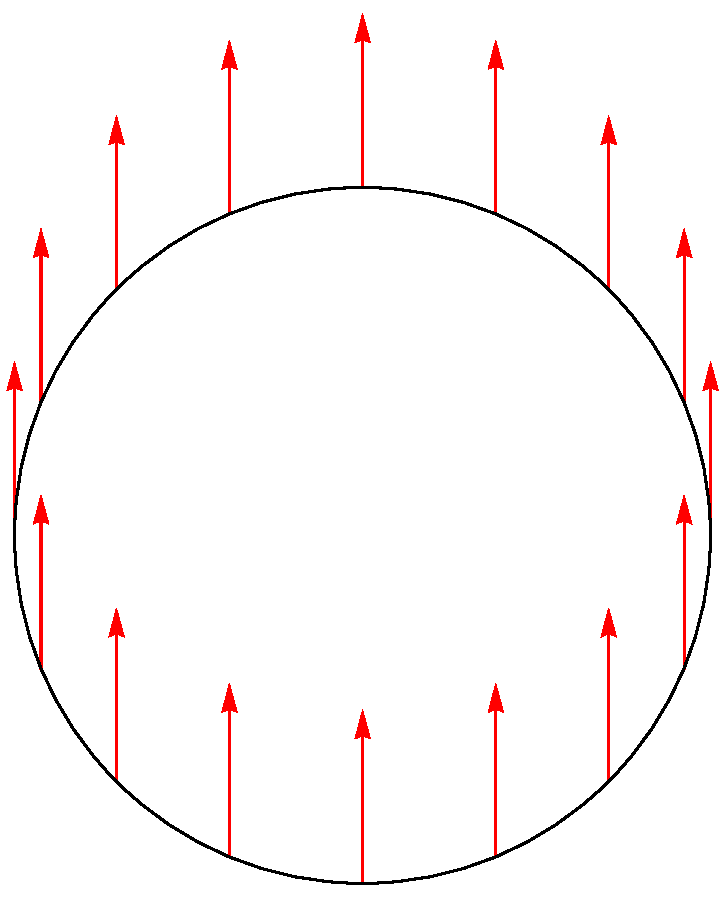
\includegraphics[scale=0.17]{lrg_gauge1.pdf} \text{(a)}  &  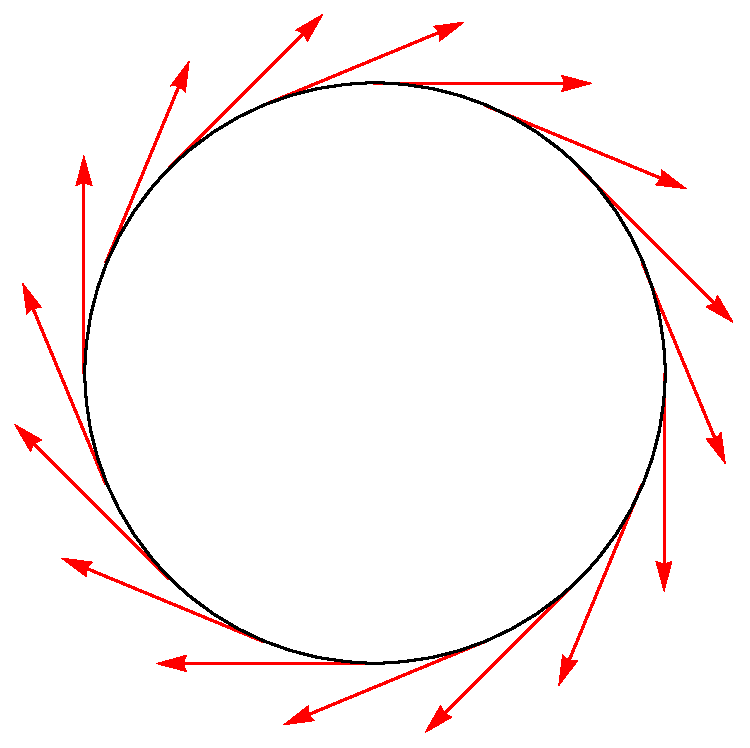
\includegraphics[scale=0.19]{lrg_gauge2.pdf} \text{(b)}  &
		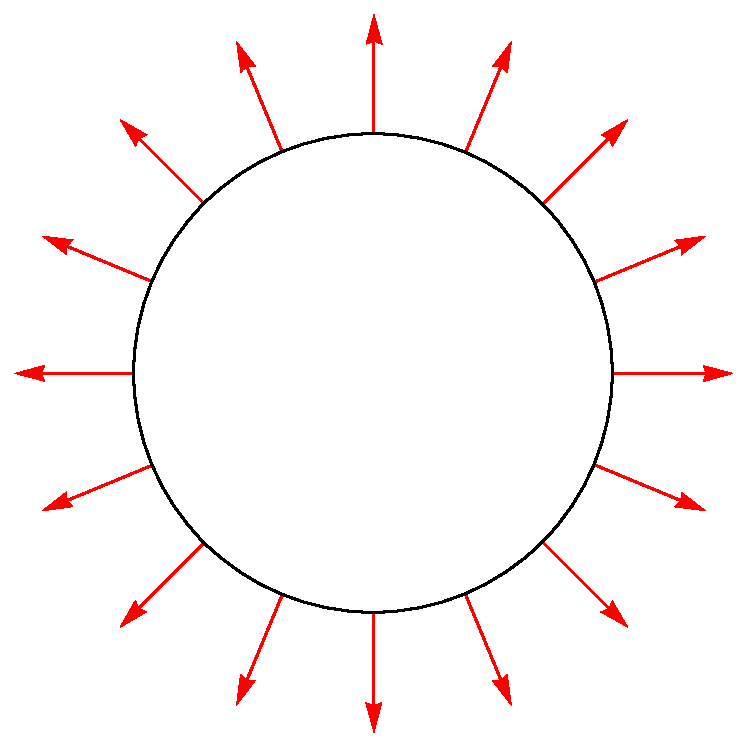
\includegraphics[scale=0.19]{lrg_gauge3.pdf} \text{(c)}
	\end{tabular}
    \caption{(a) is topologically distinct from the rest, yet they are all gauge equivalent configurations. } \label{large_gauge}
\end{figure}

As a final remark to counter the point that ``We don't live on a circle'', I shall say that when studying a non-singular circularly symmetric planar setup, we would require boundary conditions which identify the point at infinity with the same gauge-field configuration. It turns out that the point at infinity \textit{is} an $S^1$, so inevitably abelian gauge transformations \textit{would be} separated into distinct homotopy classes.

This above passage illustrates the essence of large gauge transformations in the simplest possible case, where we have a non-trivial homotopy group. The situation is precisely the same with more complicated homotopy groups but they just happen to be more difficult to visualize.

    Going back to the Lagrangian transformation law, we pick $g$, s.t. $w(g)=N$. Therefore
    \begin{align}
        S_{\text{CS}} \rightarrow S_{\text{CS } }+ 8 \pi^2 \kappa N.
    \end{align}
    Here we see that the action is \textit{not} gauge invariant! However, keep in mind that what plays a role in the path integral is $e^{i S}$, which transforms as
    \begin{align}
        e^{i S_{CS}} \rightarrow e^{i 8 \pi^2 \kappa N} e^{i S_{\text{CS}}}.
    \end{align}
    This implies that if we set $\kappa = \frac{k}{4 \pi}$, where $k\in \mathbb{Z}$, we have restored gauge invariance, which means that we ought to include this term in the study of planar physics.

    Let us look at some physical properties that the action functional $S_{\text{CS}} = \int d^3x \, \mathcal{L}_{\text{CS}}$ possesses. Performing the functional variation, we get the equation of motion $F_{\mu \nu}=0$, implying only pure gauge solutions exist. This might make one wonder, what could possibly be so interesting about CS theory if the classical equations of motion are trivial!?
    The reason that this theory is in fact interesting and non-trivial, despite the fact that $F=0$, is two-fold. Firstly, CS is a topological field theory. It has trivial local properties. All of the physics is encoded in the topology of the manifold and in the non-local observables such as Wilson loops that require us to study the full quantum theory.

    The second way in which CS is interesting teaches us the old lesson that sometimes the whole is greater than the sum of its parts. In this case, adding matter or a Maxwell term to the Lagrangian alters the pure Maxwell/matter theories immensely. Let us see how these alterations play out.

    \subsection{Chern-Simons-Maxwell Theory}
    Here we consider the familiar Maxwell theory deformed by a Chern-Simons term.
    \begin{align}
        \mathcal{L}_{\text{MCS}} &= \int d^3x \ \left[ \frac{-1}{4 g^2} F_{\mu \nu} F^{\mu \nu} + \frac{k}{4 \pi} \epsilon^{\mu \nu \rho} A_{\mu} \partial_{\nu} A_{\rho} \right]
    \end{align}
    This leads to the equations of motion
    \begin{align}
        \partial_{\mu} F^{\mu \nu} + \frac{k}{4\pi} g^2 \epsilon^{\nu \alpha \beta}F_{\alpha \beta} =0
    \end{align}
    If we rewrite this equation in terms of the dual field strength $\tilde{F}_{\mu} = \frac{1}{2} \epsilon_{\mu\nu\rho} F^{\nu\rho}$ by contracting with an $\epsilon$ tensor, followed by a $\partial$ contraction, using the equations of motion again and noting that $\partial_{\mu} \tilde{F}^{\mu} =0$ (3D Bianchi identity), we arrive at 
    \begin{align}
        \left[\partial_{\mu} \partial^{\mu} + \left(\frac{k}{2 \pi} g^2 \right)^2 \right] \tilde{F}^{\nu}=0.
    \end{align}
    Observing that $\tilde{F}^{\mu}$ is gauge-invariant, we deduce that these equations describe a propagating wave with mass $\left(\frac{k}{2 \pi} g^2 \right)$.
    Even though in this work we shall promptly be ignoring the Maxwell contribution to the planar physics, it is important to note that despite the fact that the gauge bosons are heavy, we still observe global effects. This provides us with a more general lesson about CS. Namely, that we can have significant long-rage global effects, such as the anyonic phase change interaction, even in the case of a gapped phase (such as the Quantum Hall droplet).
    Next, we turn to the matter sector.
    \subsection{Chern-Simons Matter Theory}
    
    We begin by coupling the Chern-Simons gauge field to a general conserved matter current.


    \begin{align}
        S = \int d^3x \ \frac{k}{4 \pi} \epsilon^{\mu \nu \rho} \ \mathrm{Tr} \left[A_{\mu} \partial_{\nu} A_{\rho}+ \frac{2}{3} A_{\mu} A_{\nu} A_{\rho} \right] + J^{\mu} A_{\mu}.
    \end{align}
    This action leads to a modified equation of motion.
    \begin{align}
        \frac{k}{4 \pi} \epsilon^{\mu \nu \rho} F^a_{\nu \rho} = J^{\mu}^a,
    \end{align}
    where $a=1,...,dim(\mathfrak{G})$ and $F_{\mu \nu}^a = \partial_{\mu} A_{\nu}^a - \partial_{\nu} A_{\mu}^a + [A_{\mu}, A_{\nu}]^a$. Note that covariant current conservation is equivalent to the non-abelian Bianchi identity
    \begin{align}
        D_{\mu} J^{\mu}^a = \frac{k}{4 \pi} \epsilon^{\mu \nu \rho} D_{\mu} F^{\nu \rho}^a = 0,
    \end{align}
    where $D_{\mu} F_{\nu \rho} = \partial_{\mu} F_{\nu \rho} + [A_{\mu}, F_{\nu \rho}]$.

    Restricting ourselves to the abelian case, we examine the equations of motion component by component. If $J_{\mu} = (\rho, J^i)$ then
    \begin{align}
        \rho  &= \frac{k}{4 \pi} B \label{eq:source_abel_charge} ,\\
        J^i &= \frac{k}{4 \pi} \epsilon^{i j } E_j \label{eq:source_abel_current},
    \end{align}
    where $B$ is the magnetic field perpendicular to the plane and $E_j$ is the electric field. The first equation \eqref{eq:source_abel_charge} relates the charge density to the magnetic field. So for a non-zero value of $k$, we find that anywhere there is charge, there is also magnetic flux penetrating through it perpendicular to the plane. This is something quite unlike Maxwell theory, where charge \textit{movement} generates a magnetic field, as opposed to charge \textit{presence}. This is illustrated in  Figure \ref{fig:flux_attachment} for a collection of localized charge distributions. The second equation \eqref{eq:source_abel_current} ensures that this charge-flux relation is preserved under time evolution. If we act with $\partial$ on \eqref{eq:source_abel_current} then we arrive at
    \begin{align}
        \partial_i J^i &= \frac{k}{4 \pi} \epsilon^{ij} \partial_i E_j\nonumber \\
        &= \frac{k}{4 \pi} \epsilon^{ij} \partial_i ( \partial_j A_0 - \partial_0 A_j) \nonumber \\
        &= -\frac{k}{4 \pi} \dot{B} = -\dot{\rho},
    \end{align}
    which is just the continuity equation $\dot{\rho} + \partial_i J^i=0$.





\begin{figure}[htb]
	\centering
		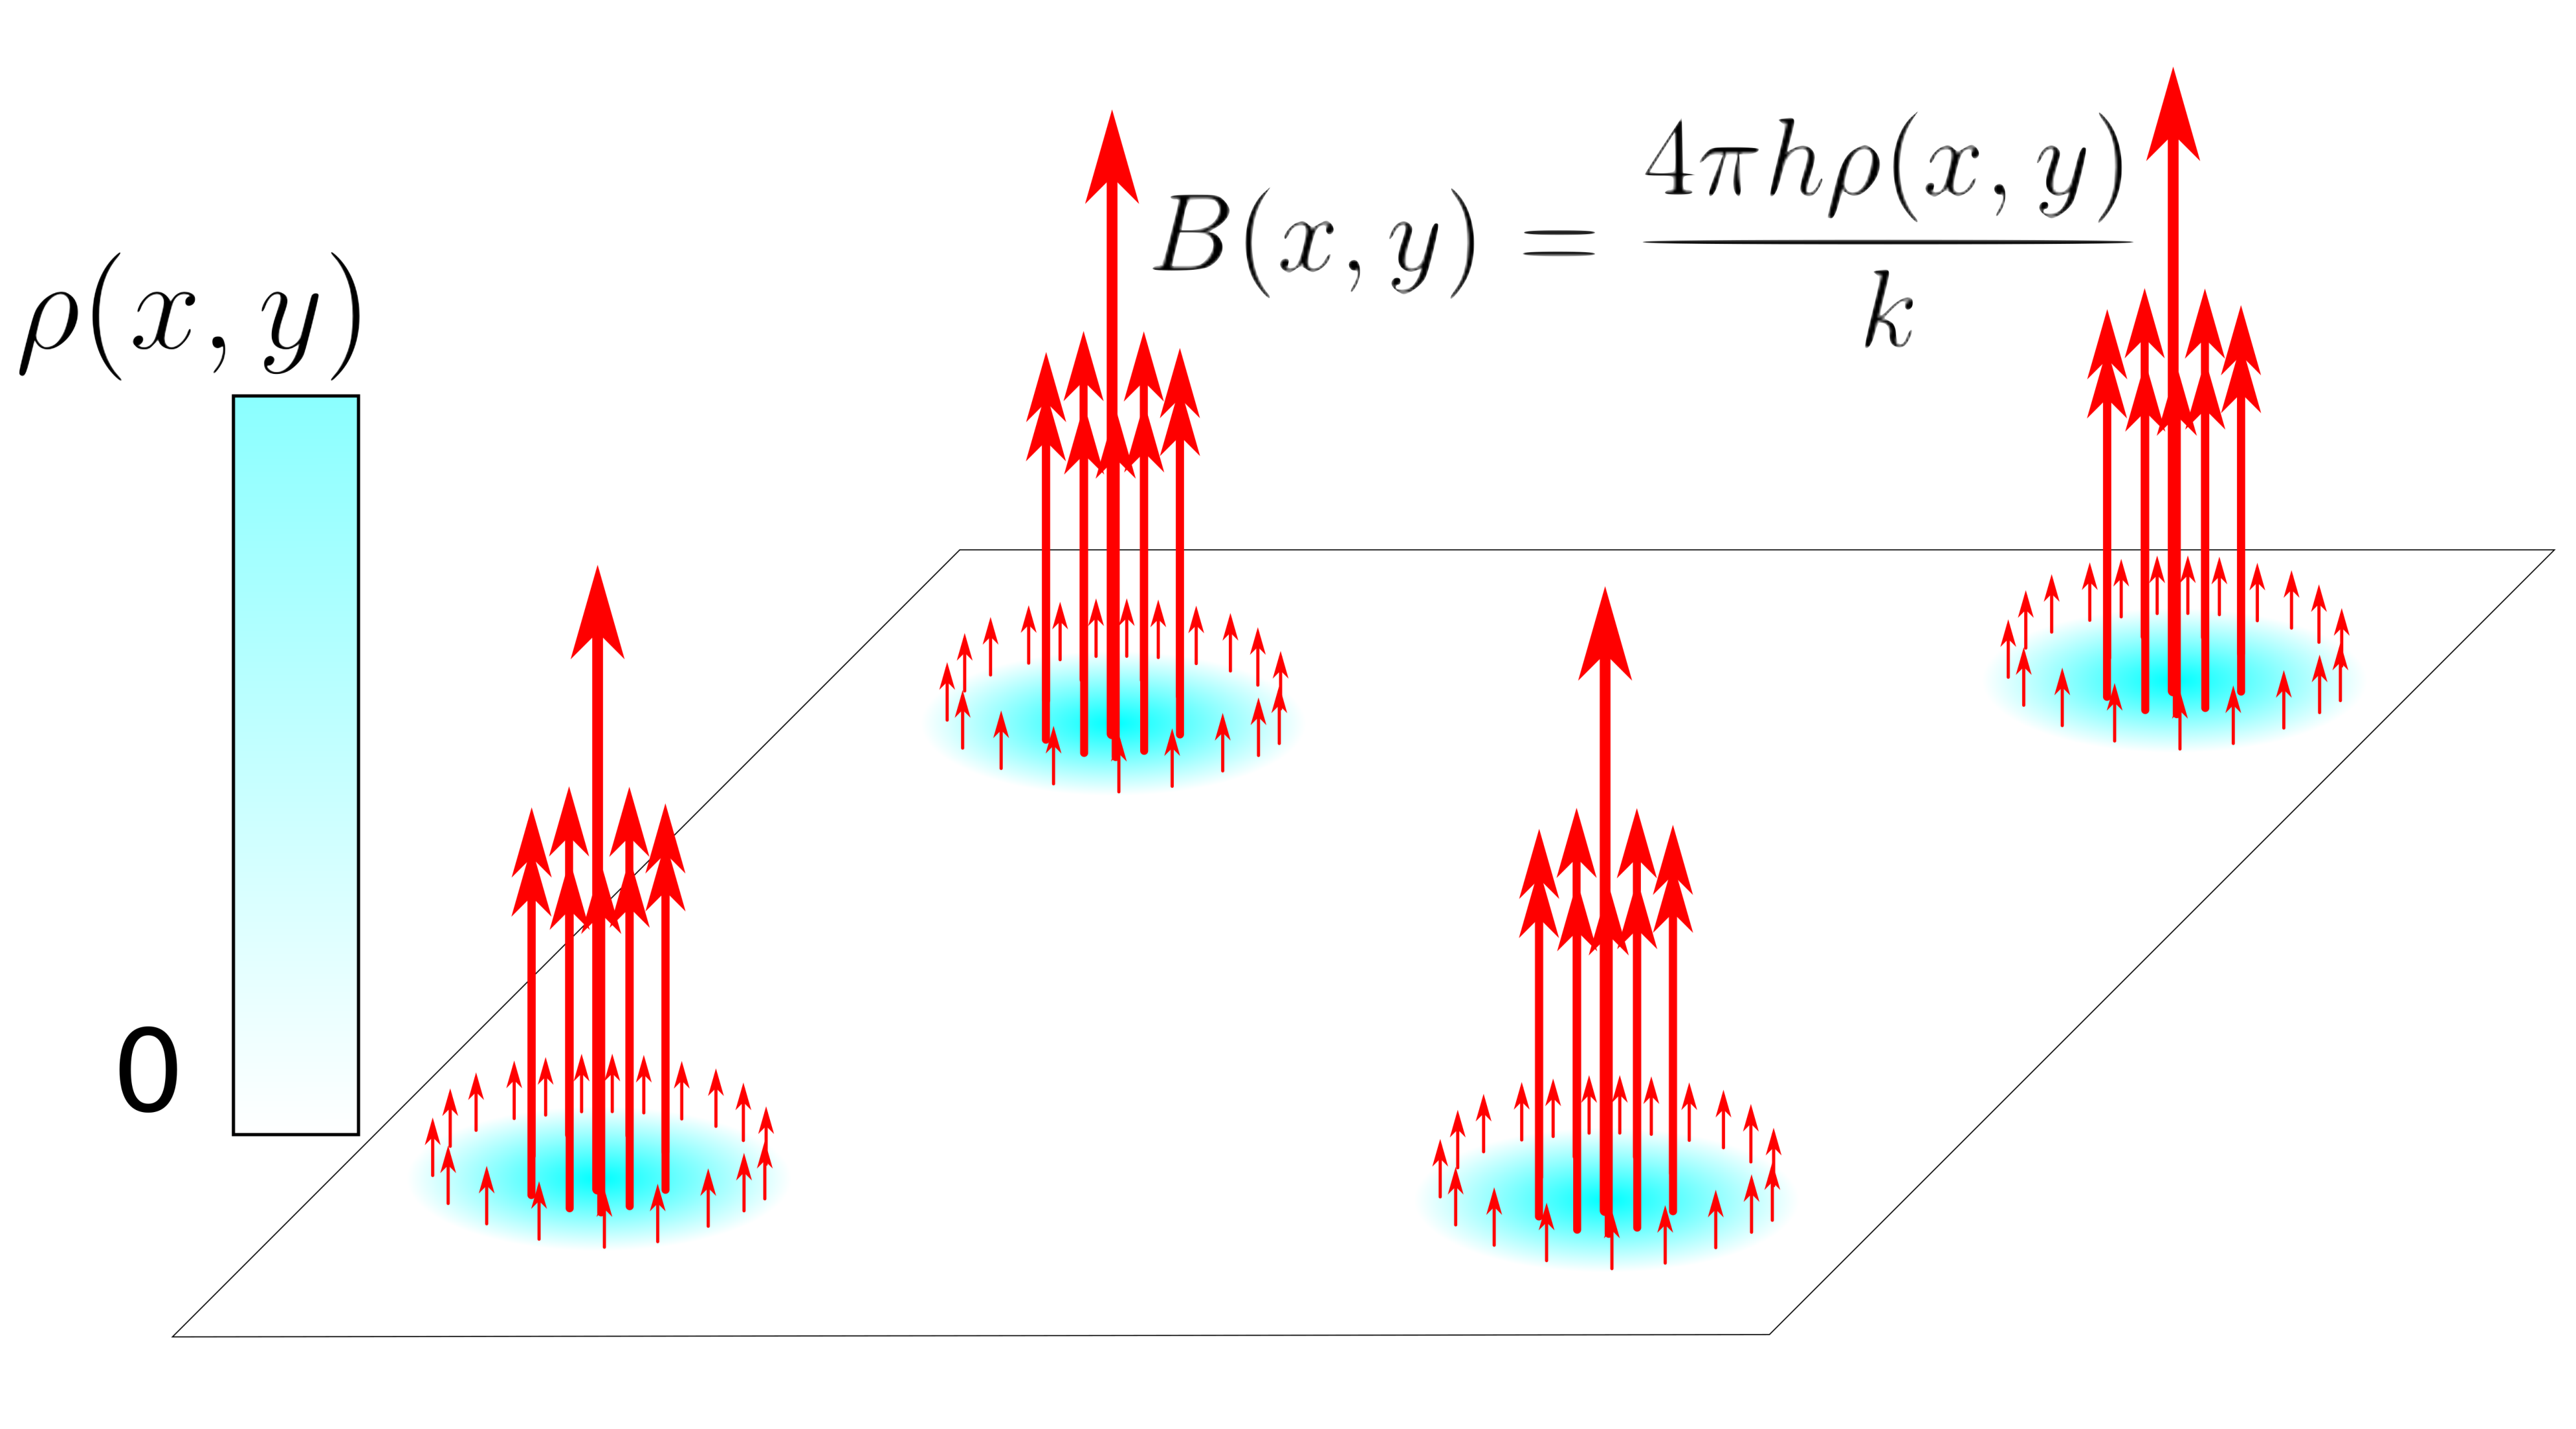
\includegraphics[scale=0.17]{Background_Folder/figures/flux_attachment_improved.pdf}
    \caption{A collection of localized charge distributions, and with magnetic flux lines of strength $\frac{4 \pi \hbar \rho(x,y)}{k}$ tied to the charges. The charge and flux are tied together throughout the motion of the particles as a result of the Chern-Simons equations \eqref{eq:source_abel_charge} - \eqref{eq:source_abel_current}.} \label{fig:flux_attachment}
\end{figure}

The final aspect of Chern-Simons theory that we will use is the fact that it is a \textit{topological} field theory (TQFT). This means that the theory is independent of the metric. This consequently implies that the CS term does not contribute to the energy-momentum tensor, since
\begin{align}
    T^{\mu \nu} = \frac{-2}{ \sqrt{-g}} \frac{\delta S_{\text{CS}}}{ \delta g_{\mu\nu}} =0.
\end{align}

One way to see that CS is a topological field theory is by writing it as an integral of a differential form.
\begin{align}
    S_{\text{CS}} &= \frac{k}{4 \pi} \int \left(A \wedge d \wedge A +A \wedge A \wedge A\right).
\end{align}
This construction does not require the metric to be defined, unlike the Yang-Mills term, which involves the hodge star (a metric dependent construct) in order to be defined through differential forms.

This concludes our review of CS theory. We now move on to a refresher of statistical physics.


        \section{Statistical Physics}

        Here we motivate the study of QFT as a gateway into understanding phenomena in many body physics. Physical phenomena at macro scale require micro scale explanations. The transition between a microscopic theory and its observable large scale properties is facillitated by the use of techniques in statistical mechanics. Here we review the connection between microscopic Lagrangian formulation and the statistical partition function through the formalism of the path integral. We follow through by accentuating the treatment of a chemical potential and the subtleties related to it. Before we go on, I note that this is the only part of this section that will be relevant to the calculations performed in this work. However, the rest of this section is meant to shine a light on why it is that we are interested in such an abstract problem.

        Upon completing this summary, we go through a short review of statistical mechanical paradigms, their successes and shortcomings. In particular, we will highlight how the Landau-Fermi liquid theory manages to do away with the complications arising from interactions and how succesful the Landau-Ginzburg symmetry breaking ideas have been in explaining large swathes of interesting phases of matter. 

        Finally, the failures of these extremely successful ideas will lead us to strongly correlated and topological systems. Notably, we discuss one system that seems to reject treatment from both of the above approaches -- a system of strongly interacting electrons confined to 2 dimensions, namely, the physical setup in which we observe the quantum hall effect. As the reader might suspect, the planar confinement is what forces us into considering CS theory as a natural candidate to explain the exotic properties of this structure.
        \subsection{Functional Integral Representation of the Partition Function}
        In this section we derive the functional integral representation of the partition function for interacting relativistic non-gauge field theories.
        Let $\hat{\phi}(\bm{x},0)$ be a Schr{\H o}dinger picture field operator at time $t=0$. We define its conjugate momentum operator to be $\hat{\pi}(\bm{x},0)$. The eigenstates of the field operator are labeled $| \phi \rangle$ and satisfy
        \begin{align}
            \hat{\phi}(\bm{x},0) | \phi \rangle = \phi(\bm{x}) | \phi \rangle,
        \end{align}
        where $\phi(\bm{x})$ is the eigenvalue of $| \phi \rangle$. This is complemented with the completeness and orthogonality relation
        \begin{align}
            \int d \phi(\bm{x}) | \phi \rangle \langle \phi | = 1, \\
            \langle \phi_a | \phi_b \rangle = \prod_{\bm{x}} \delta(\phi_a(\bm{x}) - \phi_b(\bm{x}))
        \end{align}

        And similarly for the conjugate momentum

        \begin{align}
            \hat{\pi}(\bm{x},0) | \pi \rangle = \pi(\bm{x}) | \pi \rangle, \\
            \int d \pi(\bm{x}) | \pi \rangle \langle \pi | = 1, \\
            \langle \pi_a | \pi_b \rangle = \prod_{\bm{x}} \delta(\pi_a(\bm{x}) - \pi_b(\bm{x}))
        \end{align}

        Suppose we have a Hamiltonian with no explicit time dependence


        \begin{align}
            H = \int d^2x \, \mathcal{H}(\hat{\phi}, \hat{\pi}).
        \end{align}
        Assume that a system is in a state $| \phi_a \rangle$ at time $t=0$. After a time $t_f$ it evolves to $e^{-i H t_f} | \phi_a \rangle$, assuming that the Hamiltonian has no explicit time dependence. The transition amplitude for going from state $| \phi_a \rangle$ to state $| \phi_b \rangle$ after a time $t_f$ is $\langle \phi_b | e^{-i H t_f} | \phi_a \rangle$. In order to study a system at thermodynamic equilibrium, we will be interested in the amplitude for the system returning to the same state after a time $t_f$. To be able to compute this amplitude, we divide the time interval $(0, t_f)$ into $N$ equal time steps $\Delta t = \frac{t_f}{N}$. Then at each time interval, we insert a complete set of states, alternating between field operators and their conjugate momenta


        \begin{align}
            \langle \phi_a| e^{- i H t_f} | \phi_a \rangle &= \lim_{N\rightarrow \infty} \int \left( \prod_{i=1}^{N} \frac{d\pi_i d\phi_i}{2\pi} \right) \nonumber \\
            &\times \langle \phi_a | \pi_N \rangle \langle \pi_N|  e^{-i H \Delta t}| \phi_N \rangle \langle \phi_N | \pi_{N-1} \rangle \nonumber \\
            &\times \langle \pi_{N-1} | e^{-i H \Delta t} | \phi_{N-1} \rangle \dots \nonumber \\
            &\times \langle \phi_2 | \pi_1 \rangle \langle \pi_1 | e^{-i H \Delta t} | \phi_1 \rangle \langle \phi_1 |\phi_a \rangle.
        \end{align}
        In order to evaluate this expression, we need to do several things. First of all, from single particle QM, we know that 
        \begin{align}
            \langle x | p \rangle = e^{i p \cdot x}.
        \end{align}
        So an appropriate generalization for this inner product to field operators is 
        \begin{align}
            \langle \phi_{i+1}| \pi_i \rangle = \exp \left(i \int d^2 x \ \pi_i(\bm{x}) \phi_{i+1}(\bm{x}) \right)
        \end{align}
        Since $\Delta t \rightarrow 0$, we can expand as follows, keeping terms up to first order:
        \begin{align}
            \langle \pi_i | e^{-i H_i \Delta t} | \phi_i \rangle &\sim \langle \pi_i | (1- i H_i \Delta t ) | \phi_i \rangle \nonumber \\
            &= \langle \pi_i | \phi_i \rangle (1 - i H_i \Delta t) \nonumber \\
            & = (1-i H_i \Delta t) \ \exp\left(-i \int d^2x \, \pi_i(\bm{x}) \phi_i (\bm{x})  \right),
        \end{align}
        where
        \begin{align}
            H_i = \int d^2 x \ \mathcal{H}\left(\pi_i (\bm{x}) \phi_i (\bm{x}) \right)
        \end{align}
        In the end we arrive at 
        \begin{align}
            \langle \phi_a | e^{-i H t_f} | \phi_a \rangle &= \lim_{N\rightarrow \infty} \int \left( \prod_{i=1}^N \frac{d \pi_i d\phi_i}{2\pi} \right) \delta \left(\phi_1 -\phi_a \right) \nonumber \\
            &\times \exp \left(i \Delta t \sum_{j=1}^{N} \int d^2x \left[\frac{\pi_j (\phi_{j+1} -\phi_j)}{\Delta t} - \mathcal{H}(\pi_j, \phi_j) \right] \right).
        \end{align}
        And taking the continuum limit we arrive at the path integral representation of the partition function
        \begin{align}
            &\langle \phi_a | e^{-i H t_f} | \phi_a \rangle = \int \mathcal{D} \pi \int_{\phi(\bm{x},0) =\phi_a(\bm{x})}^{\phi(\bm{x}, t_f) = \phi_a(\bm{x})} \mathcal{D} \phi \nonumber \\
            &\times \exp \left[i \int_0^{t_f} dt \int d^2 x \left( \pi(\bm{x} ,t) \frac{\partial\phi(\bm{x}, t)}{ \partial t} - \mathcal{H}\left(\phi(\bm{x},t), \pi(\bm{x},t)\right) \right) \right] \label{eq:path_integral_amplitude}.
        \end{align}
        For a Hamiltonian that is quadratic in the canonical momenta, we can just complete the square, integrate out the momenta and arrive at the usual expression for a transition amplitude in terms of a path integral over $e^{i S}$. Since our purpose here is to illuminate the connection between the statistical partition function and the path integral, we shall perform a few more manipulations. 
        \subsection{Grand Canonical Ensemble} \label{GCE_sec}
        First, we note that the grand canonical partition function is defined as follows
        \begin{align}
            Z= \tr \left[e^{-\beta \left( H - \mu N \right)}\right],
        \end{align}
        where $\beta = \frac{1}{k_b T}$ and is the inverse temperature and $\mu$ is the \textit{chemical potential}, and $N$ is a particle number. In a QFT this particle number will be associated with a conserved charge that is discretized, which is the reason why it is associated to particle number. We can express the trace in the $\phi$ basis
        \begin{align}
            Z= \int d \phi_a \langle \phi_a | e^{-\beta \left( H - \mu N \right)} | \phi_a \rangle.
        \end{align}
        We see that this expression is very similar to \ref{eq:path_integral_amplitude}. In order to match the two expressions, we need to do three things. First, we set $t \rightarrow -i \tau$, such that $t_f \rightarrow -i \beta$. Then we shift the Hamiltonian density in order to account for the inclusion of a chemical potential
        \begin{align}
            \mathcal{H} \left(\phi(\bm{x},t),\pi (\bm{x},t) \right) \rightarrow \mathcal{H}\left(\phi(\bm{x},t),\pi (\bm{x},t) \right) - \mu \ \mathcal{N}\left(\phi(\bm{x},t),\pi (\bm{x},t) \right),
        \end{align}
        where $\mathcal{N}$ is a number density. Finally, we include the trace operation, which integrates over all possible boundary conditions. In the end we are left with
        \begin{align}
            Z &= \int \mathcal{D} \pi \int_{\text{periodic}} \mathcal{D} \phi \exp \left[ \int_0^{\beta} \int d^2x \left(\pi \frac{\partial \phi}{\partial t} - \mathcal{H}(\pi, \phi) + \mu \mathcal{N}(\pi, \phi) \right) \right] \label{eq:partition_function}.
        \end{align}
This is the path integral representation of the partition function of the grand canonical ensemble of a single real scalar field. This expression is readily generalizable to more fields by integrating over the extra fields and their respective conjugate momenta.

Here we shall make a few observations that will come in use frequently for the rest of this work. For the purposes of presentation, we will elaborate on these points in the context of a somewhat simpler model. This should not alarm the reader, because the properties we are discussing are more general and model independent. With this in mind, we consider the Lagrangian description of a complex relativistic scalar in $2+1d$ with a potential $U(\phi)$.
        \begin{align}
            \mathcal{L} = \left(\partial_{\mu}\phi^{*} \partial^{\mu} \phi  - U\big(|\phi|\big)\right).
        \end{align}
        This system possesses a global symmetry
        \begin{align}
            \phi \rightarrow e^{i \alpha} \phi, \qquad\qquad \phi^* \rightarrow e^{-i \alpha} \phi^*.
        \end{align}
        This leads to a conserved Noether current and consequently a conserved charge
        \begin{align}
            J_{0} &= -i \int d^2x \left( \pi \phi - \pi^{\dag}\phi^{\dag}\right),
        \end{align}
        where $\pi = \frac{\delta \mathcal{L}}{\delta ( \partial_0 \phi)}$ is the canonical momentum. Based on the assumption of identical particles with discrete charges, we postulate that $J_0 = \mathcal{N}$. Next, we perform the momentum integrals in \eqref{eq:partition_function}. Since now we have a complex field, we have to integrate over all of $\phi$, $\phi^{\dag}$, $\pi$ and $\pi^{\dag}$.
        \begin{align}
            Z &= \int \mathcal{D} \pi \mathcal{D} \pi^{\dag} \int_{\text{periodic}} \mathcal{D} \phi \mathcal{D} \phi^{\dag} \nonumber \\
            &\times \exp \left[ \int_0^{\beta} \int d^2x \left(\pi \frac{\partial \phi}{\partial t} +\pi^{\dag} \frac{\partial \phi^{\dag}}{\partial t} - \mathcal{H}(\pi, \pi^{\dag}, \phi, \phi^{\dag}) - i  \mu \left(\pi \phi - \pi^{\dag}\phi^{\dag} \right) \right] \label{eq:partition_function_complex_scalar} \nonumber \\
            &= \int \mathcal{D} \pi \mathcal{D} \pi^{\dag} \int_{\text{periodic}} \mathcal{D} \phi \mathcal{D} \phi^{\dag} \nonumber \\
            &\times \exp \left[ \int_0^{\beta} \int d^2x \left(\pi \left( \frac{\partial \phi}{\partial t} -i \mu \phi \right) +\pi^{\dag} \left( \frac{\partial \phi^{\dag}}{\partial t} +i \mu \phi^{\dag} \right) - \mathcal{H}(\pi, \pi^{\dag}, \phi, \phi^{\dag})  \right] \label{eq:partition_function_complex_scalar}
        \end{align}
        Performing the path integral leaves us with
        \begin{align}
            Z= \int_{\text{periodic}} \mathcal{D}\phi \mathcal{D}\phi^{\dag} \exp \left[\int_0^{\tau} d\tau \int d^2x \mathcal{L'} \right],
        \end{align}
        where $\mathcal{L'}$ is the same as $\mathcal{L}$ except for the time derivatives acting on $\phi$ now act as covariant derivatives in the presence of a constant background gauge field $A_0=\mu$, \ie
        \begin{align}
            \partial_0 \rightarrow \partial_0 -i \mu. \label{eq:chemical_potential_gauge_field}
        \end{align}
        This is a general result that we will be making use of numerous times.
        \subsubsection{Chemical Potential for a Local Symmetry}
        Now, let us see how this situation changes when we try to introduce a chemical potential for a gauged symmetry. First, we modify the Lagrangian $\mathcal{L}$ by gauging the $U(1)$ and adding a Maxwell term $-\frac{1}{4 g^2} F_{\mu \nu} F^{\mu \nu}$. For simplicity, let us assume that the potential has the monomial super-renormalizable form
        \begin{align}
            U\big(|\phi| \big) = \lambda |\phi|^4.
        \end{align}
        Therefore
        \begin{align}
            \mathcal{L} &=( D_{\mu} \phi)^* D^{\mu} \phi - \lambda |\phi|^4 - \frac{1}{4 g^2}F_{\mu \nu} F^{\mu \nu},
        \end{align}
        where $D_{\mu}= \partial_{\mu} - i A_{\mu}$. According to the rule \ref{eq:chemical_potential_gauge_field} that we established above , 
        \begin{align}
            \mathcal{L} \rightarrow \mathcal{L}'= \mathcal{L}\left(\phi,\ D_{\mu}' \phi,\ A_{\mu} \right),
        \end{align}
        where $D_{\mu}' = D_{\mu} - i \mu \delta_{\mu 0}$.
        Let us also express $\phi$ in terms of a modulus and a phase
        \begin{align}
            \phi(x) = \sigma(x) e^{i \alpha(x)}.
        \end{align}
        If we assume a homogenous, constant configuration, the equations of motion tell us that
        \begin{align}
            \sigma &= \sqrt{\frac{\mu^2}{2\lambda}}  \label{eq:chem_pot_local_symmetry_eom1} \\
            \frac{1}{g^2} \partial_{\mu} F^{\mu 0} &= \mu \sigma^2. \label{eq:chem_pot_local_symmetry_eom2}
        \end{align}
        The first equation tells us that the scalars have condensed to the ground state. The second equation states that we have a non-zero charge density in this ground state. On the one hand, this makes sense, since the charged scalars have condensed. On the other hand, this is contradictory, since we are studying a system at equilibrium. And a charged system cannot be in equilibrium by definition. In order to fix this problem, we introduce a background charge density, which guarantees that the system is neutral.
        \begin{align}
            \mathcal{L}' \rightarrow \mathcal{L}' - A_0 J_0,
        \end{align}
        where $J_0 = \frac{\mu^3}{2\lambda}$.

        %\subsection{Physical Applications}\label{phys_app_sec}
        %\subsubsection{Landau-Fermi Liquid Theory} \label{Fermi_Liquid_sec}
        The statistical description of weakly interacting particles, for example, in a fluid can be thought of as the same as that of a free gas of non-interacting quasiparticles that are in one to one correspondence with the original interacting excitations of the material. We find that in order to explain some of the surprising feature of the charge carriers in a QH system, we need to go beyond the weakly interacting description of a Landau-Fermi liquid.
        %\subsubsection{Landau-Ginzburg Paradigm} \label{Landau-Ginzburg_sec}
        %\textcolor{red}{***More to add***} \\
        %- Introductory part talk about the problem of scales, how mean field theory tackles the problems well away from the critical temperature, but at the critical point, all scales need to be taken into account. We are left with a LG functional that no longer contains information about the microscopic system -- we find a universal effective theory describing said phenomenon.
        %- Symmetry breaking \\
        %- Order parameters\\
        %- The Girvin MacDonald ``Landau-Ginzburg''-like model. \cite{Girvin1987} In 1987, Girvin \& MacDonald proposed a LG effective model to describe the FQHE. \\
        %- Read's improvement \cite{Read1989}\\
        %- The Zhang, Hansson, Kivelson microscopic Hamiltonian improvement \cite{PhysRevLett.62.82}
        \section{Fractional Quantum Hall Effect} \label{FQHE_sec}
        Here we discuss what is perhaps the most applied aspect of TQFT in the real world. But before we get to the point of discussing the highly non-trivial physics of the various types of Quantum Hall Effects, we take a moment to review the classical picture.
        \subsection{Classical Hall Effect}
        In the year 1879, Edwin Hall set up an experiment consisting of a conductor plate with two electrodes attached at either end of it, generating a current, and a magnetic field penetrating the surface of the conductor perpendicularly. He found that he could measure a non-zero potential across the conductor, orthogonal to the plane defined by the driving current and the magnetic field. The generation of this potential difference has since been known as the \textit{Hall effect}. Despite this being an exciting discovery at the time, from our modern perspective this is all accounted by basic knowledge of conductors and classical electrodynamics. In the presence of a magnetic field, the charge carriers, which are responsible for the current in the conductor, get deflected in a direction orthogonal to their motion due to the Lorentz force
        \begin{align}
            F = q(\bm{E} + \bm{v}\times \bm{B}),
        \end{align}
        where $q$ is the charge of the electrons, $\bm{E}$ is the electric field due to the potential difference in the electrodes, $\bm{v}$ is the velocity of the charge carriers and $\bm{B}$ is the magnetic field in the material. If we were to account for the possible collisions that may occur within a sample of the conductor, which will cause the charge carriers (in this case electrons) to slow down, we shall arrive at a slightly modified equation to the Lorentz law from above
        \begin{align}
            m \dot{\bm{v}} = q \bm{E}+q \bm{v}\times \bm{B} - \frac{1}{\tau} m \bm{v}, \label{eq:Drude_Model_Background}
        \end{align}
        where $\tau$ is the \textit{scattering time} -- it accounts for how frequently the electrons scatter, hence a large scattering time makes the term disappear completely. This description of the charge carriers in a material, subject to both electric and magnetic field, in the presence of impurities, is called the \textit{Drude model}, named after the German physicist Paul Drude, who first proposed it. Before we look at the general solution of this model, we make several remarks about certain limiting cases.\\
        \indent First, assume that there are no collisions (\textit{i.e.} the collision time diverges $\tau \rightarrow\infty$) and that there is no electric field. Then the system simplifies to
        \begin{align}
            m\dot{\bm{v}} =q \bm{v}\times \bm{B}.
        \end{align}
        For a particle confined to the plane the velocity vector is $\bm{v} = (\dot{x}, \dot{y})$, which leads to the system of two coupled linear ODEs
        \begin{align}
            m \ddot{x} = q B \dot{y}, \qquad m \ddot{y}= -q B \dot{x}.
        \end{align}
        The general solution to this system is
        \begin{align}
            x(t) &= x_0 + R \sin\left(\omega_Bt + \varphi \right) \\
            y(t) &= y_0 + R \cos\left(\omega_Bt + \varphi \right),
        \end{align}
        where $x_0, y_0, R, \varphi$ are all integration constants and
        \begin{align}
            \omega_B = \frac{q B}{m}
        \end{align}
        is the \textit{cyclotron frequency}.
        We that the solution in the absence of collisions and an electric potential is circular motion with a fixed magnetic field dependent frequency.\\
        Let us go back to the full Drude model. We would like to find out what the equilibrium of the system looks like. This implies that $\dot{v} =0$. The equation of motion becomes 
        \begin{align}
            \bm{v} - \frac{q \tau}{m}\bm{v}\times\bm{B}  &=\frac{\tau q}{m} \bm{E} \\
            \begin{bmatrix}
                1 & -\frac{q \tau B}{m} \\
                \frac{q \tau B}{m} & 1 \\
            \end{bmatrix} \bm{v} &= \frac{\tau q}{m} \bm{E}.
        \end{align}
        Subsituting $\bm{J} = q \bm{v}$ and $\omega_B = \frac{q B}{m}$
        \begin{align}
            \begin{bmatrix}
                1 & -\omega_B \tau \\
                \omega_B \tau & 1 \\
            \end{bmatrix}\bm{J} = \frac{\tau q^2}{m} \bm{E}.
        \end{align}
        After inverting we arrive at \textit{Ohm's law}
        \begin{align}
            \bm{J}=\sigma \bm{E},
        \end{align}
        where
        \begin{align}
            \sigma=\frac{q^2 \tau }{m \left(\tau ^2 \omega_B ^2+1\right)}
\begin{bmatrix}
 1 & \tau  \omega_B  \\
 -\tau  \omega_B  & 1 \\
\end{bmatrix}
        \end{align}
         is the \textit{conductivity} tensor. It is related to the \textit{resistivity} tensor by
         \begin{align}
            \rho = \sigma^{-1}= \frac{m}{q^2 \tau } \begin{bmatrix}
 1 & -\tau  \omega_B  \\
 \tau  \omega_B  & 1 \\
            \end{bmatrix} = \begin{bmatrix}
                \rho_{xx} & \rho_{xy} \\
                \rho_{yx} & \rho_{yy} \\
            \end{bmatrix},
         \end{align}
         where $\rho_{xx} =\rho_{yy}$ and $\rho_{xy} = - \rho_{yx}$.

         This equation tells us that in the presence of a constant magnetic field, the charge carriers experience two types of resistivity. One is the usual type of resistivity that you can expect from a conductor $\rho_{xx} = \frac{m}{q^2\tau}$ -- It is independent of the magnetic field and as the scattering time increases, \textit{i.e.} the number of scattering events decreases, the resistivity decreases. The other type of resistivity is different. The off-diagonal component of the resistivity $\rho_{yx} = \frac{m \omega_B}{q^2}= \frac{B}{q}$ is independent of $\tau$. So somehow the resistivity in the direction orthogonal to that of the driving current does not depend on the impurities in the material. Another way in which $\rho_{yx}$ is different is that it depends on the magnetic field. Surprisingly, as $B\rightarrow 0$ so does $\rho_{yx} \rightarrow 0$. It would be incorrect to assume that the vanishing of $\rho_{xy}$ implies that we achieve superconductivity, since $\sigma_{xy}$ also vanishes so there is no current being generated perpendicular to the generating electric field.

        The Drude model is successful when compared to the classical experimental results obtained by Hall since it predicts correctly that the resistivity  $\rho_{xy}$ would grow linearly with the magnetic field $B$.
        \subsection{Quantum Hall Effect}
        Now that we have an understanding of the classical Hall effect we are ready to delve into the physics of the quantum hall effect. It's important to distinguish two different types of quantum Hall effects, since they are qualitatively different, occur in different materials and seem to have fundamentally different physical explanations.
        The first type is the Integer Quantum Hall effect. In 1980, Klaus von Klitzing was performing the Hall experiment at ultralow temperatures with strong magnetic fields and found that the above relation between $\rho_{yx}$ and $B$ does not hold for large enough magnetic fields. He found that beyond a certain magnetic field strength, plateaux started appearing in the resistivity that could not be explained by the classical picture. Further, he found that in the plateaux, where $\rho_{yx}$ was constant, $\rho_{xx}$ was vanishing. The precise relation that he discovered was
        \begin{align}
            \rho_{yx} = \frac{2 \pi \hbar}{e^2} \frac{1}{\nu}, \qquad \nu \in \mathbb{Z}.
        \end{align}
        Thus the quantity $\frac{2 \pi \hbar}{e^2}$ is dubbed the quantum of resistivity. The explanation of the Integer Quantum Hall effect is based on the quantum mechanics of non-interacting particles confined to a plane. In the case of the fractional quantum hall effect (FQHE), where $\nu \in \mathbb{Q}$, we need to study a highly interacting system, which makes the FQHE a very interesting topic for theoretical physics.

        Our exploration of the Quantum Hall Effect will stop here. What is important to take away from this section is that the understanding of the FQHE is underlied by the study of Chern-Simons theory. Thus studying the models, that are of interest in the present work, might lead to a better understanding of the fascinating problem that is the FQHE. A further connection to this problem is provided by the non-commutative Chern-Simons theory that we explore at the end of this chapter and at the end of chapter 3. Next, we turn our attention to the study of vortices.

%\textcolor{red}{***More to add***}\\
%        - Drude Model
%        - Classical electrodynamic explanation of classical Hall effect\\
%        - Integer Quantum Hall effect \\
%   \indent         - discovered by von Klitzing\\
%        - Fractional Quantum Hall effect\\
%    \indent        - Leads to charge fractionalization\\
%           \indent - Laughlin wave function
        \section{Vortices} \label{vortices_sec}
        This section takes up the task of summarizing basic aspects about vortices in general and specifically in Chern-Simons matter theories.
        Vortices are localized, exact solutions to the equations of motion. They may or may not be finite energy configurations.
        In 1957, Abrikosov  showed that if the surface tension between two phases of matter (in his case those were superconducting and non-superconducting phases) is negative, then a phase transition would be accompanied by the creation of a lattice of regions, whose interiors reside in a phase different from their exteriors \cite{Abrikosov1957}. He also recognized the similarity between these regions of non-superconductivity have with the vortices formed in superfluid helium. This similarity is due to the winding of the phase of the order parameter wave function.


        Later on, in 1973, Nielsen \& Olesen \cite{Nielsen1973} showed that a solution similar to that of Abrikosov can come about through the study of a microscopic Lagrangian, as opposed to in an effective Landau-Ginzburg description. This is the Lagrangian of the abelian Higgs model with a quartic interaction. Similar solutions have been found in the abelian Higgs model with a Chern-Simons interaction by Paul-Khare \cite{Paul1986} and in the absence of a Maxwell term by Hong-Kim-Pac \cite{Hong1990}, Jackiw and Weinberg \cite{Jackiw1990a} and Jackiw, Lee and Weinberg \cite{Jackiw1990b}.

        \subsection{Global U(1) Vortex}

        Now we look at the properties of these solutions more closely. Before we look at the gauge theory scenario, we focus on the simplest case of a complex massive scalar with a fourth order interaction, negative mass squared and a global $U(1)$ symmetry

        \begin{align}
            \mathcal{L} &=  \left|\partial_{\mu} \phi \right|^2 + m^2 | \phi |^2 - \lambda |\phi|^4.
        \end{align}
    This leads to the equations of motion
    \begin{align}
        \partial_{\mu} \partial^{\mu} \phi = m^2 \phi - 2\lambda |\phi|^2 \phi
    \end{align}
    This system has an $S^1$ vacuum manifold, parametrized by $\phi = v e^{i \theta}$, where $\theta \in [0,2\pi)$ is the planar polar angular coordinate and $v^2 = \frac{m^2}{2 \lambda}$. We may consider a field configuration that is $\phi=0$ at the origin but approaches a different point on the vacuum manifold at spatial infinity depending on $\theta$. More precisely, we are looking at a field $\phi$ such that
    \begin{align}
        \phi \xrightarrow[]{r\rightarrow \infty} v e^{i n\theta},
    \end{align}
    where $n \in \mathbb{Z}$ in order to guarantee that the physical configuration is single-valued.
    We would like to compute the energy of such a static circularly symmetric configuration

    \begin{align}
        E= 2 \pi \int_0^{\infty} r dr \left[\lambda |\phi|^4 - m^2 |\phi|^2 + |\phi'|^2 + \frac{n^2 v^2}{r^2} \right].
    \end{align}
    Close to infinity, the potential term vanishes and so does $\phi'$. In the end we are left with
    \begin{align}
        E = 2\pi n^2 v^2 \int \frac{dr}{r} =  2\pi n^2 v^2  \ \log R,
    \end{align}
    where $R$ is the sample size on which our theory is defined. We see that the global vortex, if it exists, would only have a finite energy for finite samples and is not well-defined in the most general case. It turns out that once the global symmetry is gauged, the divergence disappears and we have a vortex configurations that is well defined in the infinite volume limit.

        \subsection{Local U(1) Vortex}
        The gauged $U(1)$ vortex, also known as the Abrikosov-Nielsen-Olesen vortex is again a configuration that interpolates between two different vacua in a theory, but this time we introduce a gauge field, whose dynamics is governed by a Maxwell term and is minimally coupled to a $U(1)$ scalar with a symmetry breaking potential. This is the familiar abelian Higgs model. 
        \begin{align}
            S_{\text{AH}} & = \int d^3x \left[-\frac{1}{4} F_{\mu \nu} F^{\mu \nu} + | D_{\mu} \phi|^2 - U(\phi) \right], \label{eq:Abelian_Higgs_Model}
        \end{align}
        where
        \begin{align}
            U(\phi) = \frac{\lambda}{2} |\phi|^4 - m^2 |\phi|^2.
        \end{align}
    Again, we have non-trivial manifold of ground states and we can repeat the construction from above. This time the energy of the static radially symmetric configuration ends up slightly different.
    \begin{align}
        E = 2 \pi \int_0^{\infty} r dr \left(\frac{1}{2}( B^2 + E^2) + |D_{\mu} \phi|^2 + U(\phi) \right)
    \end{align}
    This time we are aiming for eliminating the divergence that arose from the kinetic term $|\partial_{\mu}\phi|$ by requiring that $A_{\mu}$ asymptotes to a value that cancels it, in such a way that this value can be arrived at through a gauge transformation, ensuring that at $r\rightarrow \infty$, $A_{\mu}$ is pure gauge, thus yielding a finite contribution from the electromagnetic field. Such a choice for $A_{\mu}$ is
    \begin{align}
        A_{\mu} = n \partial_{\mu} \alpha(x),
    \end{align}
    where $\alpha(x) = \theta$. Hence
    \begin{align}
        A_0 =0, \qquad A_r =0, \qquad A_{\theta} = n.
    \end{align}
    This implies that
    \begin{align}
        \int_0^{\infty} r dr |D_{\mu}\phi|^2 = v^2\int_0^{\infty} r dr  \frac{1}{r^2}|n-A_{\theta}|^2 =0.
    \end{align}
    From here we see that the inclusion of a gauge field has cured the divergence and we are left with a sensible infinite volume limit. 

    Now that we know that these boundary conditions do not lead to a divergence in the energy, let us see whether a solution with such boundary conditions exists. We write down the equations of motion.
    \begin{align}
        \frac{1}{g^2}  \partial_{\rho}(r F^{\mu \rho}) = i r \left[\phi^* \left(D^{\mu}\phi\right) - \left(D^{\mu}\phi \right)^* \phi \right] \nonumber \\
        \partial_{\mu} \left(r D^{\mu} \phi \right) - i A_{\mu} D^{\mu} \phi + \frac{\delta U}{\delta \phi^*} =0
    \end{align}
    After substituting the ansatz
    \begin{align}
        \phi = \sqrt{\frac{m^2}{\lambda}}v(r) e^{i n \theta}, \qquad A_{\mu} = n a(r) \delta_{\theta \mu},
    \end{align}
    and rescaling $r\rightarrow \frac{\hat{r}}{m}$, we arrive at a system of equations for the dimensionless functions $v(r)$ and $a(r)$.
    \begin{align}
        \frac{1}{\hat{r}} \frac{d }{d \hat{r}} \left(\hat{r} \frac{d v}{d \hat{r}} \right) - \frac{n^2 (a-1)^2 v}{\hat{r}^2} -v^3 +v =0  \\
        \frac{d}{d \hat{r}}\left(\frac{1}{\hat{r}}\frac{d}{d \hat{r}} a \right)- \frac{2 g^2}{\lambda r} (a-1)v^2=0.
    \end{align}
    In these variables, the boundary conditions become
    \begin{align}
        v(0) = 0, \qquad a(0)=0, \\
        v(\infty) =1, \qquad a(\infty) =1.
    \end{align}


    For small $r$, the solutions to these equations look like
    \begin{align}
        v(r)&= J_n(r) \sim \frac{r^n}{ 2^n n!} \\
        a(r)&= C r^2
    \end{align}
    And asymptotically for large $r$ we have

    \begin{align}
        v(r)&=K_0\left(\sqrt{2} r\right)\sim 2^{-\frac{3}{4}}\sqrt{\frac{\pi}{r}} e^{- \sqrt{2} r} \\
        a(r)&=r K_1\left(\frac{\sqrt{2} g}{\sqrt{\lambda}} r \right)\sim 2^{- \frac{3}{4}} \sqrt{\frac{\pi r \sqrt{\lambda}}{g}} e^{- \sqrt{2} \frac{g}{\sqrt{\lambda}}r}
    \end{align}

    From here we can recover the masses of the gauge field and Higgs field $m_{H}$ and $m_a$, respectively, in the Higgsed phase of the theory.
    \begin{align}
        m_{H}= \sqrt{2} m, \qquad m_a = \sqrt{2} \frac{g^2}{\lambda}m
    \end{align}
    From the from of the propagator for scalar and vector theories, we know that scalar fields act attractively, whereas gauge fields act repulsively for like-charged configurations. This tells us that when $m_a>m_H$, the gauge field decays slower than the scalar field, so if we were to place two vortices on the plane, we will observe an attractive force between them. Likewise, if  $m_a<m_H$, we expect the vortices to repel each other. This line of thought hints at us that there is a critical value of the couplings, where vortices are free (non-interacting). Here we present a more precise argument for this. In order to do this, we will Bogomol'nyi's identity.

    \begin{align}
        |D_1 \phi|^2 + |D_2 \phi|^2 = |D_1 \phi \pm D_2 \phi|^2 \pm B |\phi|^2. \label{eq:Bogomolnyi}
    \end{align}
    Further, we re-express the potential by completing the square.

    \begin{align}
        U(\phi)&=\frac{\lambda}{2} \left( |\phi|^2 - v^2 \right)^2 - \frac{m^2 v^2}{2}. \label{eq:potential_square}
    \end{align}
    Here we can ignore the constant since the energy is defined up to a constant (albeit an infinite one). Utilizing \eqref{eq:Bogomolnyi} and \eqref{eq:potential_square} we reach the following expression for the energy of this configuration

    \begin{align}
        E &= 2 \pi \int r dr \bigg(\frac{1}{2 g^2}B^2 \pm B(|\phi|^2 -v^2) + \frac{\lambda}{2} \left(|\phi|^2 -v^2 \right)^2 \\ \nonumber 
        &+ |D_1\phi \pm i D_2 \phi|^2 \pm B v^2 \bigg) \\ \nonumber
        &= 2 \pi \int r dr \bigg[|D_1\phi \pm i D_2 \phi|^2 +\frac{1}{2}\left( \frac{B}{g} \pm \lambda \left(|\phi|^2 -v^2  \right) \right)^2   \\ \nonumber \\
        &\pm \left(1 - \frac{\sqrt{\lambda}}{g} \right) B \left(|\phi|^2 - v^2 \right) \bigg] \pm n v^2,
    \end{align}
    where we have used Stokes' theorem.

    \begin{align}
        \int r dr B = n.
    \end{align}

    In order to have no interaction between the vortices, we need the energy of the $n$ vortex, the bound state of n vortices, to be the same as the energy of $n$ separate vortices. This implies that there is no potential energy, hence no force between them. This condition is satisfied when

    \begin{align}
        |D_1\phi \pm i D_2 \phi|^2 =0&,  \qquad \frac{B}{g} \pm \lambda \left(|\phi|^2 -v^2  \right) =0, \label{eq:BPS1_Abel}\\
        \lambda &= g^2 .\label{eq:BPS2_Abel}
    \end{align}
    The above equations (\eqref{eq:BPS1_Abel} and \eqref{eq:BPS2_Abel}) are known as the BPS equations of the vortex, named after the people who first discovered a non-interacting limit for solitonic solutions in field theory -- Bogomol'nyi, Prasad and Sommerfield \cite{Bogomolny:1975de} \cite{Prasad1975}.
    
\begin{figure}[htb]
	\centering
	\begin{tabular}{c@{\hspace{1.5cm}}c@{\hspace{1.5cm}}c}
        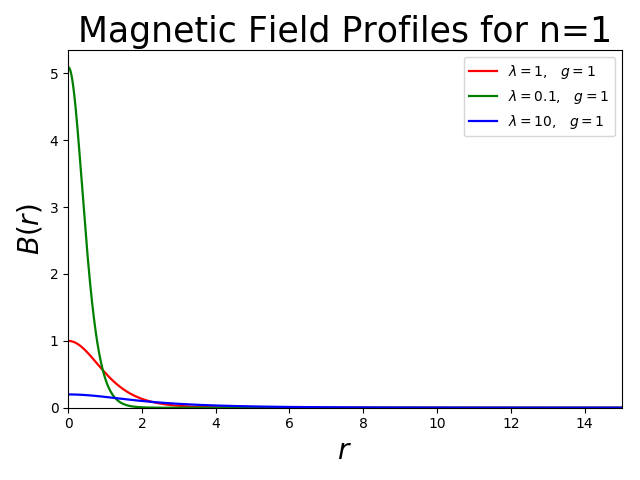
\includegraphics[scale=0.4]{Background_Folder/figures/solution_n1_magnetic_field_g_lambda.png}
        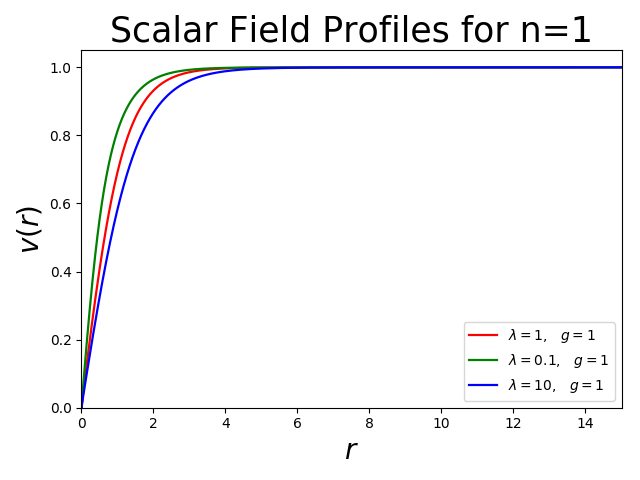
\includegraphics[scale=0.4]{Background_Folder/figures/solution_n1_scalar_field_g_lambda.png}
	\end{tabular}
    \caption{Scalar and magnetic field profiles for n=1 and $\lambda = (10,1,0.1)* \lambda_c$} \label{plot:Abelian_Higgs_Profiles_n1}
\end{figure}

    \subsection{Particle-Vortex Duality}
    The considerations of the previous section are more general and they apply for more than just systems in $2+1d$ even though the details differ. In a general QFT, we have roughly two different types of quantum excitations. One is the familiar type of elementary excitations that appear through the standard procedure of canonical quantization, where we introduce creation and annihilation operators that insert particles at a given position. The other type is, as we have just seen from the previous section, of a \textit{solitonic nature} (such as vortices). In other words, a solution that we reach not through expanding around the free solution in a small coupling parameter, but is more generally associated with a stationary point parametrically far from the free theory. This makes these solutions grow in size and energy the smaller the coupling is so studying them in the quantum regime becomes tricky. Luckily, because their masses become large at small coupling, they decouple from the theory so one can study the quantum theory of the elementary excitations on its own without worrying about the solitons. Unfortunately, going in the other direction in terms of coupling strength, the solitons become light and their importance grows but so do quantum corrections for the elementary excitations and we reach a regime, where we do not understand the theory. So how do we learn more about these strongly coupled theories?

    One approach that has become ever more popular in the past few decades is the idea of a \textit{duality}. Duality suggests that instead of having one model or one Lagrangian that describes the physics of a system, we instead have two. For example, a way in which duality can manifest itself is the following. Theory \textit{I} has elementary excitations that we can study at weak coupling and non-perturbative excitations which are inaccessible due their large mass. Whereas theory \textit{II} describes the solitons of theory \textit{I} as its own elementary excitations at weak coupling (and a small mass) and the solitons present in theory \textit{II} are in fact the elementary states of theory \textit{I}. If the non-perturbative states in these systems are vortices in $2+1$ dimensions, then we have a type of Strong-Weak duality called a \textit{Particle-Vortex duality}. 

    Since we now have a reasonable grasp of what vortices are, we are ready to introduce particle-vortex duality. And what better place to start than the Abelian Higgs model from the last section \eqref{eq:Abelian_Higgs_Model}. Earlier we saw that non-perturbative solutions exist in this theory. It turns out that a model exists where the vortices of the Abelian Higgs model appear as elementary excitations. In other words, there is a duality between these two models
    \begin{align}
        S_{\text{AH}} \longleftrightarrow S_{\text{XY}},
    \end{align}
    where
    \begin{align}
        S_{\text{XY}} &= \int d^3x |\partial_{\mu}\tilde{\phi}|^2-m^2 |\tilde{\phi}|^2 - \frac{\tilde{\lambda}}{2} |\tilde{\phi}|^4.
    \end{align}
    $S_{\text{XY}}$ is the action for the so called \textit{XY model} and $S_{\text{AH}}$ is defined as in \eqref{eq:Abelian_Higgs_Model}. The matching of the physics in the different phases is summarized in table \eqref{table:PV_Duality}.

    \begin{table}
\begin{center}
  \begin{tabular}{| l | c | c | c|}
      \hline
    $m^2$ & $<0$ & $=0$ & $>0$\\ \hline
     & Coulomb phase &  & SB phase\\ 
    $S_{\text{XY}}$ & $2d$ logarithmic & WF fixed point & local ANO \\ 
     & potential &  & vortices \\ \hline
      & SB phase &  &  Massive excitations\\
    $S_{\text{AH}}$ & global vortices & WF fixed point & in\\
      & $E\xrightarrow{V \rightarrow \infty} \infty$ &  & Coulomb phase \\
    \hline
  \end{tabular}
\end{center}
      \caption{This table shows the matching of the phases of the XY model and the Abelian Higgs model}
        \label{table:PV_Duality}
    \end{table}
In \cite{1606.01893}, the authors showed a link between this particle-vortex duality and bosonization. This naturally leads us to the next section, which focuses on Fermi-Bose duality.


%\textcolor{red}{***More to add***}\\
%-- Say something about the relation between particle-vortex duality and bosonization \cite{1606.01893, 1606.01912} \\
%Some history, Abrikosov \cite{Abrikosov1957}, type $I$ and $II$ superconductors. Vortices are solitons -- this means that they are non-perturbative solutions to the equations of motion that are localized and stable.\\
%            - Topological vs Non-Topological\\
%            - Review other vortices such as Abrikosov, Abelian Higgs, Pure Chern-Simons, Non-abelian vortices
%

%    \begin{itemize}
%        \item Tong TASI Solitons \cite{hep-th/0509216}
%        \item Importance of BPS \cite{Bogomolny:1975de, Prasad1975}
%    \end{itemize}
        \section{Fermi-Bose Duality} \label{Fermi-Bose_sec}
        We already met the idea of duality in the previous section. In general, they tend to be an equivalence of two theories. Two different ways in which we can state the same physics. Some of them are functional integral analogs of the Fourier transform (for functionals) -- one phenomenon can be described either in coordinate or momentum space, by one action or another. This can be achieved by introducing a Lagrange multiplier field and integrating out the original fields. Others tend to arise in consequence of the idea of universality. Two models that flow to the same CFT in the IR will tend to be equivalent sufficiently close to the fixed point.
        Yet other types of duality are inspired by the study of black hole thermodynamics and the holographic principle, such as the AdS/CFT duality. Others still, seem to be a consequence of deep mathematical ideas, such as the level-rank duality.

        Whatever the fundamental reasons for their existence is, dualities are interesting becase they give us another point of view that allows us to explore and understand the world of fundamental physics in more depth. As Feynman once said, ``Every theoretical physicist who is any good knows six or seven different theoretical representations for exactly the same physics''\cite{Feynman_quote}. And in the spirit of his words, here duality is one more representation we wish to understand.\\
        \indent As pointed out above, dualities come in many flavours and the models we are considering here play a role in more than one type. $O(N)/U(N)$ (scalar or fermion) models are holographically dual to higher spin gravitational theories \cite{hep-th/0210114}. This duality seems to persist even after deforming the theories with a Chern-Simons term in the large $N$ limit\cite{1110.4382}. Fermions in 2+1d can be shown to be dual to vector fields via a Fourier transform-like functional integral transformation that we described above \cite{hep-th/9401105, Barci1996}. And pure Chern-Simons theories are level-rank dual to each other \cite{Naculich1990, Camperi1990, Mlawer1991, Nakanishi1992, hep-th/0703089}. In this section, we will concentrate on a duality that has all of the above ingredients in some form ($SU(N)/U(N)$ scalars/fermions and CS vector fields) that combine into what's believed to be an IR duality. More precisely, we are talking about a set of dualities between $2+1d$ gauge theories that are collectively known as \textit{Fermi-Bose duality}.\\
        \indent The duality between fermions and bosons was first conjectured  in the supersymmetric context\cite{0808.0360, 1108.5373, 1305.3924, 1411.5475}. Evidence for the non-supersymmetric version of these dualities comes from large $N$ computations on both sides both at finite temperature \cite{1211.4843}  and at $T=0$ \cite{1110.4386}. Furthermore, there is compelling evidence that the duality holds at finite $N$ from supersymmetric theories flowing to their non-SUSY versions \cite{1305.7235, 1507.04378}.\\
        \indent Since $U(N) = (SU(N)\times U(1))/\mathbb{Z}_N$, we can in principle have different Chern-Simons levels for the $SU(N)$ and $U(1)$ symmetries. We will denote a $U(N)$ Chern-Simons theory with levels $k_1$ and $k_2$ corresponding to the $SU(N)$ and $U(1)$ symmetries, respectively, as a $U(N)_{k_1,k_2}$ theory. Prior to the inclusion of matter in our model, we state an important fact about these theories. Namely, that some choices of gauge groups and levels are dual to others. This is known as \textit{level-rank duality}. It's generalization to include matter is the duality that we present below. In Yang-Mills regularization the Fermi-Bose dualities are as follows \cite{1512.00161}.
            \begin{align}
                SU(N)_k + scalars &\longleftrightarrow \ \ U(k)_{-N +\frac{N_f}{2}, -N + \frac{N_f}{2}} \quad + fermions,  \\
                U(N)_{k,k} + scalars &\longleftrightarrow SU(k)_{-N +\frac{N_f}{2}}\qquad \ \ \ \quad+ fermions,  \\
                U(N)_{k,k+N} + scalars &\longleftrightarrow \ \ U(k)_{-N +\frac{N_f}{2}, -N + \frac{N_f}{2}-k} \ + fermions.  
            \end{align}
            The scalars on the LHS of these equations are assumed to be tuned to a critical interacting point of the RG flow, known as the Wilson-Fisher fixed point. (Explain how the Wilson Fisher fixed point work). Similarly to PV duality, which maps elementary excitations to non-perturbative vortices, Fermi-Bose duality maps the fundamental perturbative states on one side to monopole or baryon operators on the other side. \\
            \indent Understanding the details of this duality subject to the inclusion of a chemical potential has been the formative motivation for this work. We believe that some of the results of this thesis have sown the seed for this understanding. More specifically, the role of the ground state discussed in chapter 3 in the duality still remains mysterious. The resolution of this mystery is left for future work. Thus we conclude our discussion of Fermi-Bose duality and move on to the physics of non-commutative fluids
%\textcolor{red}{***More to add***}\\
%            - Make sure to include the first bosonization papers \cite{hep-th/9407078, hep-th/9407182} \\
%            - Explain what is the precise dictionary of this duality. The two theories are equivalent but which degrees of freedom correspond to which. Clarify that fundamental perturbative states on one side map to monopole operators on the other and vice-versa.\\
%            - Monopole operators
%
        \section{Non-Commutative Fluids}
    In this section we will define important physical notions in a non-commutative geometry, show how it relates to the theory of fluids and demonstrate how the non-commutative version of the Landau problem leads directly to the non-commutative Chern-Simons action. Finally, we discuss the Fock space of this action to prepare the presentation of results that we have discovered. For a good summary of this topic, we refer the reader to this set of excellent reviews on physics on non-commutative geometry \cite{0706.1095, hep-th/0109162, hep-th/0106048}.

    Non-commutative geometry can arise naturally from the quantization of a particle's phase space coordinates. The simplest way to see this connection is through the Heisenberg algebra of the canonical commutation relations. 
    \begin{align}
        [\hat{x}, \hat{p}] = i \hbar.
    \end{align}
    As is well known, this quantization condition leads to a ``smearing out`` of the phase space structure of the theory. It makes it so that the notion of a point in phase space no longer makes sense, since one can no longer measure both position and momentum accurately. \\
    \indent However, there are more exotic cases, where the coordinate space becomes non-commutative or fuzzy, due to the specific form of the Poisson brackets in the problem. In such a problem, the notion of a point in space is no longer reasonable and one can no longer measure the position of a (quasi)particle to arbitrary accuracy on both axes at once. An example of a problem, where the different momenta exhibit such non-commutativity is the problem of particles in a magnetic field that we discussed earlier. Similarly, we all know that angular momentum also behaves in a non-commutative way so the idea of the spatial coordinates having non-zero commutator comes naturally. Finally, in the study of fluids, one can define a type of Poisson bracket that is restricted to the coordinate space, which leads to a non-commutative space following a canonical quantization \cite{Jackiw2002}. These ideas of a non-commuting space-time were first explored by Snyder in 1947 \cite{Snyder1947_space_time, Snyder1947_EM}.


    \subsection{Review of Non-Commutative Geometry}
    Let us see how to define a \textit{non-commutative space}. Here we will be concerned with a $D$ dimensional space-time that has both a set of $D-2p$ commuting $\{ y_i, \ i=2p+1,...,D\}$ and $2p$ non-commuting coordinates $\{ x_i, \ \alpha =1,...,2p\}$. More precisely,
    \begin{align}
        [y_i, y_j] &=0\\
        [x_{\alpha}, x_{\beta}] &=i \bm{\theta}_{\alpha \beta}, \label{eq:space_time_commutations}
    \end{align}
    where $\theta$ is an anti-symmetric constant one-form. One can perform linear transformations on the coordinates $x_{\alpha}$ so that the matrix $\theta$ is in canonical block form

    \begin{align}
        \bm{\theta}_{\alpha \beta } = \theta \begin{bmatrix}
            i \bm{\sigma_2} &  & \text{\huge0} \\
                     & \ddots &  \\
                    \text{\huge0} &  & i \bm{\sigma_2} \\
                \end{bmatrix},
    \end{align}
    where 

    \begin{align}
        i \bm{\sigma_2} = \begin{bmatrix}
            0 & 1 \\
            -1 & 0 \\
        \end{bmatrix}.
    \end{align}

    This leaves us with $p$ pairs of the Heisenberg algebra
    \begin{align}
        [x_{2\alpha -1}, x_{2\alpha}]=i\theta, \qquad \alpha=1,...,p.
    \end{align}
    This quantization of the spatial coordinates leads to the existence of a Hilbert space. Since we can now think of the coordinates as operators, then each operator has a set of eigenstates with associated quantum numbers. To make this more explicit, let us define the \textit{creation}, \textit{annihilation} and \textit{number} operators
    \begin{align}
        \bm{a}_{\alpha} = \frac{x_{2\alpha-1} +i x_{2\alpha}}{\sqrt{2 \theta}}, \qquad \bm{a}^{\dag}_{\alpha} &= \frac{x_{2\alpha-1} -i x_{2\alpha}}{\sqrt{2 \theta}} \\
        \bm{n}_{\alpha} = \bm{a}^{\dag}_{\alpha}\bm{a}_{\alpha}.
    \end{align}
    These operators allow us to build the familiar \textit{Fock space} from QFT by acting on a vacuum state
    \begin{align}
        |n_1,...,n_p\rangle=  \bm{a}^{\dag}_1^{n_1}... \bm{a}^{\dag}_p^{n_p}|0\rangle
    \end{align}

    Further, we define the derivative operators through the relations
    \begin{align}
        \partial_{\mu} \cdot x_{\nu} = [\partial_{\mu}, x_{\nu}] = \delta_{\mu \nu}, \qquad \mu,\nu = 1,...,D.
    \end{align}
    Specifically for the non-commuting coordinates
    \begin{align}
        \partial_{\alpha}= -i \omega_{\alpha \beta} x_{\beta}, \qquad \alpha, \beta = 1,...,2p.
    \end{align}
    where $\omega_{\alpha \beta} = \left(\theta^{-1} \right)_{\alpha \beta}$. From here it follows that
    \begin{align}
        [\partial_{\alpha}, \partial_{\beta}] = i \omega_{\alpha \beta}.
    \end{align}


    \subsection{Non-Commutative Field Theory}

    Now that we understand some of the basic ideas of non-commutative geometry, we would like to define a field theory on this non-commutative space. The simplest possible gauge theory contains just a gauge field $A_{\mu}$. Further, the easiest way to construct a gauge invariant theory is by forming an action that is composed of a trace of covariant derivatives 
    \begin{align}
        D_{\mu} = -i \partial_{\mu} + A_{\mu},
    \end{align}
    since under a gauge transformation $D_{\mu}$ transforms as
    \begin{align}
        D_{\mu} \rightarrow U D_{\mu} U^{-1}.
    \end{align}
    Restricting ourselves to the non-commuting submanifold, we have
    \begin{align}
        D_{\alpha} &= -i \partial_{\alpha} + A_{\alpha} = \omega_{\alpha \beta}x^{\beta}+ A_{\alpha} = \omega_{\alpha \beta} \left( x^{\beta}+ \theta^{\beta \gamma} A_{\gamma} \right) \equiv \omega_{\alpha \beta} X^{\beta}.
    \end{align}
    

    \\ 
    - Specifically, non-commutative Chern-Simons theory arises as the action of a massless particle confined to the plane in the presence of a magnetic field. \cite{hep-th/0103013} Let us take a look at the action of a particle of charge $q$ and mass $m$ moving in an electromagnetic field generated by the four-potential $A^{\mu} = \left(-V(\bm{x}, t), \ \bm{A}(\bm{x},t)\right)$
    \begin{align}
        S = \int dt \left(\frac{1}{2} m^2 v^2 - q V(\bm{x},t) + q \bm{v} \cdot \bm{A}(\bm{x},t)\right). \label{eq:Lagrangian_Charged_Particle_In_EM_Field}
    \end{align}
    Now, let us assume that the particle is massless and in addition, it is in a constant magnetic field and the electric potential is 0. Since $\nabla \times \bm{A} = \bm{B}$, this implies that
    \begin{align}
        A_i = \frac{B}{2} \epsilon_{i j} x_j,
    \end{align}
    where $B= |\bm{B}|$.
    Substituting this expression into \eqref{eq:Lagrangian_Charged_Particle_In_EM_Field}
    \begin{align}
        S = \int dt \left( q \frac{B}{2}\epsilon_{i j} \dot{x_i} x_j \right).
    \end{align}
    From here we proceed by making the identification
    \begin{align}
        x_i \leftrightarrow X_i.
    \end{align}
    And since the $X_i$'s transform under gauge transformations, we ought to make sure that the action remains invariant. To this end, we need to also gauge the time derivative $\partial_0 \rightarrow D_0 = \partial_0 +A_0$
    \begin{align}
        S = \int dt \ \left[ q \frac{B}{2} \epsilon_{ij} Tr \left(D_0 X^i X^j \right) \right] = \int dt \ \left[ q \frac{B}{2} \epsilon_{ij} Tr \left(\partial_0 X^i X^j + [A_0, X^i] X^j \right) \right]
    \end{align}
    The introduction of the time component of the gauge field leads to a Gauss's law constraint
    \begin{align}
        [X^1, X^2] =0.
    \end{align}
    It seems that this constraint has removed the non-commutativity that we tried to introduce into our model. In order to bring it back, we add an extra term to the action such that we get the Heisenberg algebra \eqref{eq:space_time_commutations} that we explored earlier
    \begin{align}
        S =\int dt \ \left[ q \frac{B}{2} \epsilon_{ij} Tr \left(\partial_0 X^i X^j + [A_0, X^i] X^j + 2 \theta A_0 \right) \right].
    \end{align}
    Thus we have arrived at the non-commutative abelian Chern-Simons model by considering the movement of charged particles in a magnetic field confined to a two-dimensional plane.

    

